\newthought{\textbf{Resha Russita - 2020903430040 - TRKJ 3B}}

\newday{\textbf{1 - 2 Desember 2022} - Instalasi dan Konfigurasi Hadoop}
\begin{enumerate}
\item Kendala dan Solusi
\newline Pada Instalasi Apache Hadoop, saya sebagai praktikan mengalami kendala saat mengekstrak file Apache Hadoop. Solusi yang saya gunakan adalah membuat kembali os ubuntu dengan ukuran ruang yang lebih besar dari sebelumnya sehingga file yang diekstrak berhasil. 
Kendala lain yang terjadi adalah hanya kurang teliti saat melakukan konfigurasi pada Apache Hadoop.

\begin{figure}[!ht]
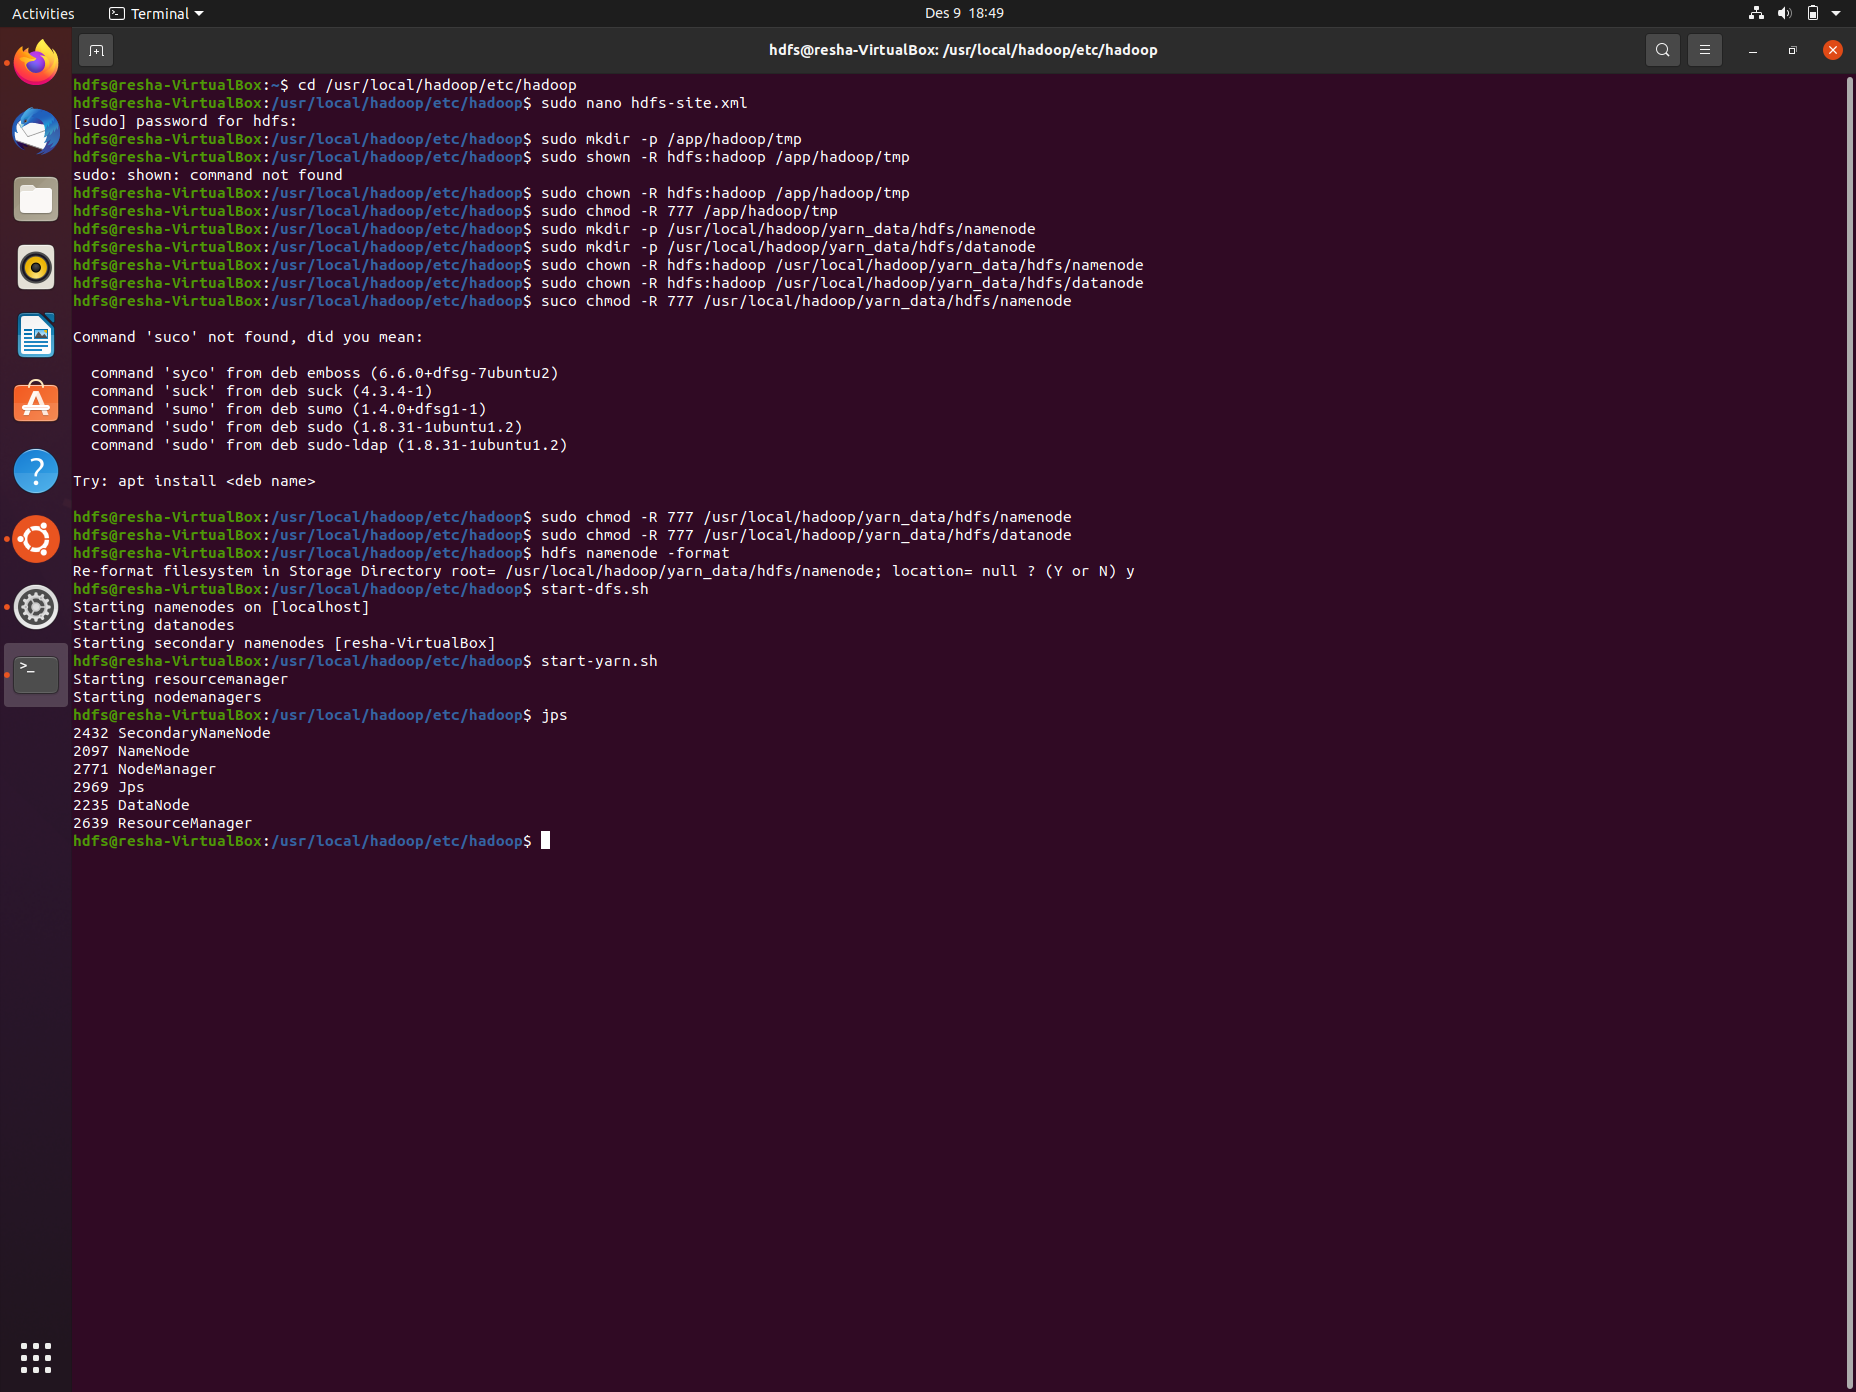
\includegraphics[width=.9\textwidth]{ReshaRussita/jpshadoopservice-resha}
\caption{cek services hadoop dengan jps}
\label{gam:perkuliahan-22-09}
\end{figure}

\begin{figure}[!ht]
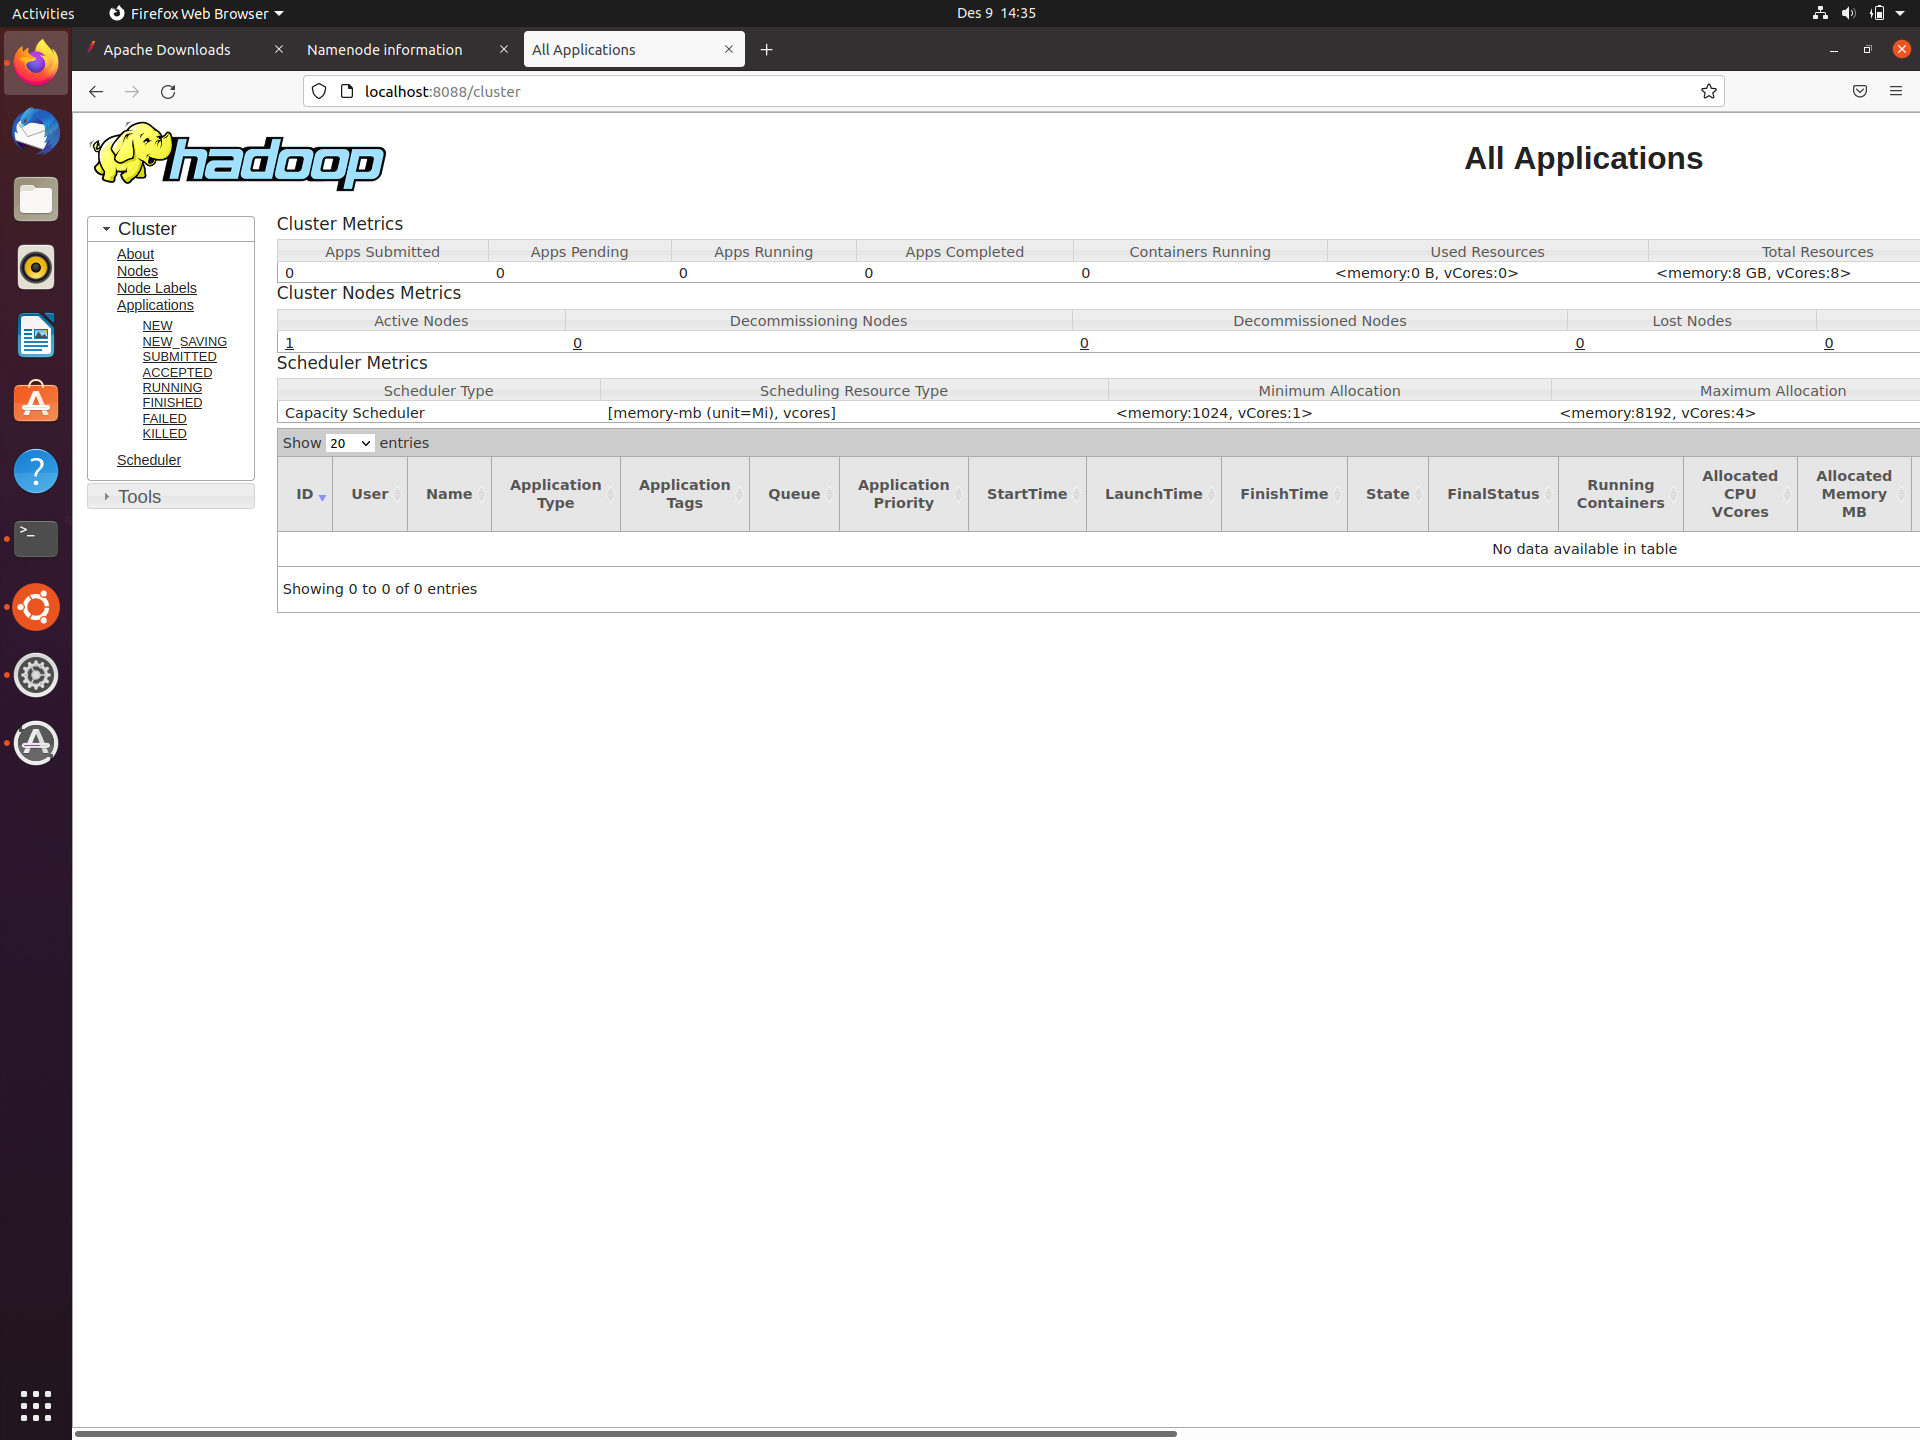
\includegraphics[width=.9\textwidth]{ReshaRussita/localhost8088-resha}
\caption{local host 8088 akses}
\label{gam:perkuliahan-22-09}
\end{figure}

\begin{figure}[!ht]
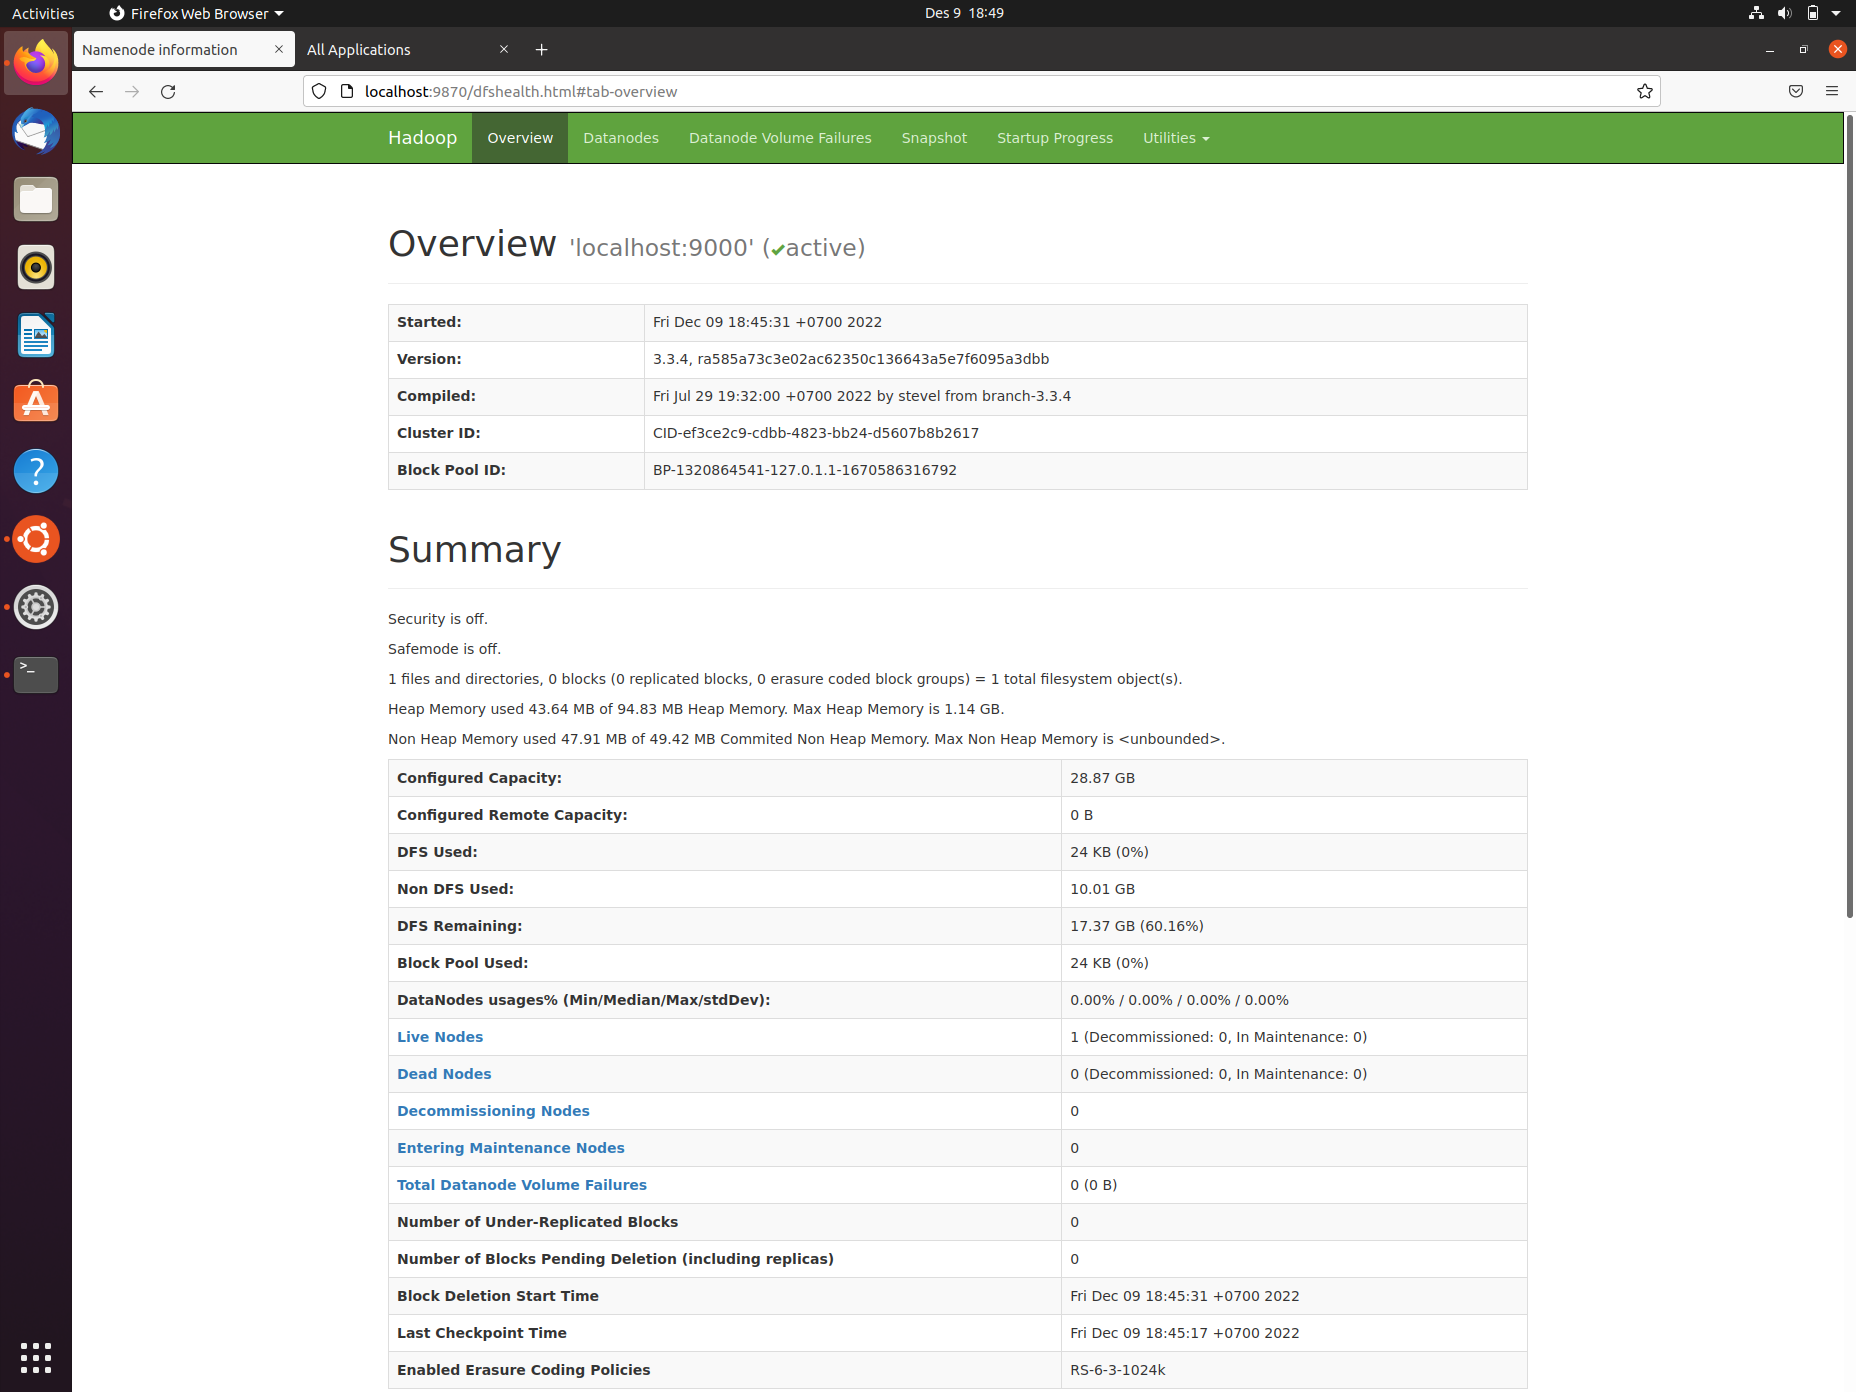
\includegraphics[width=.8\textwidth]{ReshaRussita/localhost9870-resha}
\caption{local host 9870 akses}
\label{gam:perkuliahan-22-09}
\end{figure}

\newpage
\item Kesimpulan
\newline Pada Instalasi Apache Hadoop membutuhkan ruang yang cukup besar untuk mengekstrak file Apache Hadoop. Penginstalaan Apache Hadoop harus dilakukan sesuai step, begitu juga pada saat konfigurasi. Konfigurasi ini bertujuan untuk memudahkan user dalam memonitoring ekosistem di dalam Hadoop. Saat mengkonfigurasi terdapat perintah untuk membuat format HDFS yang berfungsi menyimpan suatu data dengan cara membaginya menjadi potong-potongan data yang disebut blok berukuran 64 MB dan kemudian disimpan pada node-node yang tersebar dalam kluster. Node-node yang ada adalah name node dan data node. Sehingga saat mengecek Hadoop service dengan perintah jps, kedua node tersebut harus tersedia sebagai pendukung saat dilakukan akses web browser dengan local host 9870 dan 8088 itu berhasil.
\end{enumerate}


\newday{\textbf{8 Desember 2022} - WordCount bawaan Hadoop}
\begin{enumerate}
\item Kendala dan Solusi
\newline Pada program WordCount bawaan Hadoop, tidak ada kendala yang saya alami.

\begin{figure}[!ht]
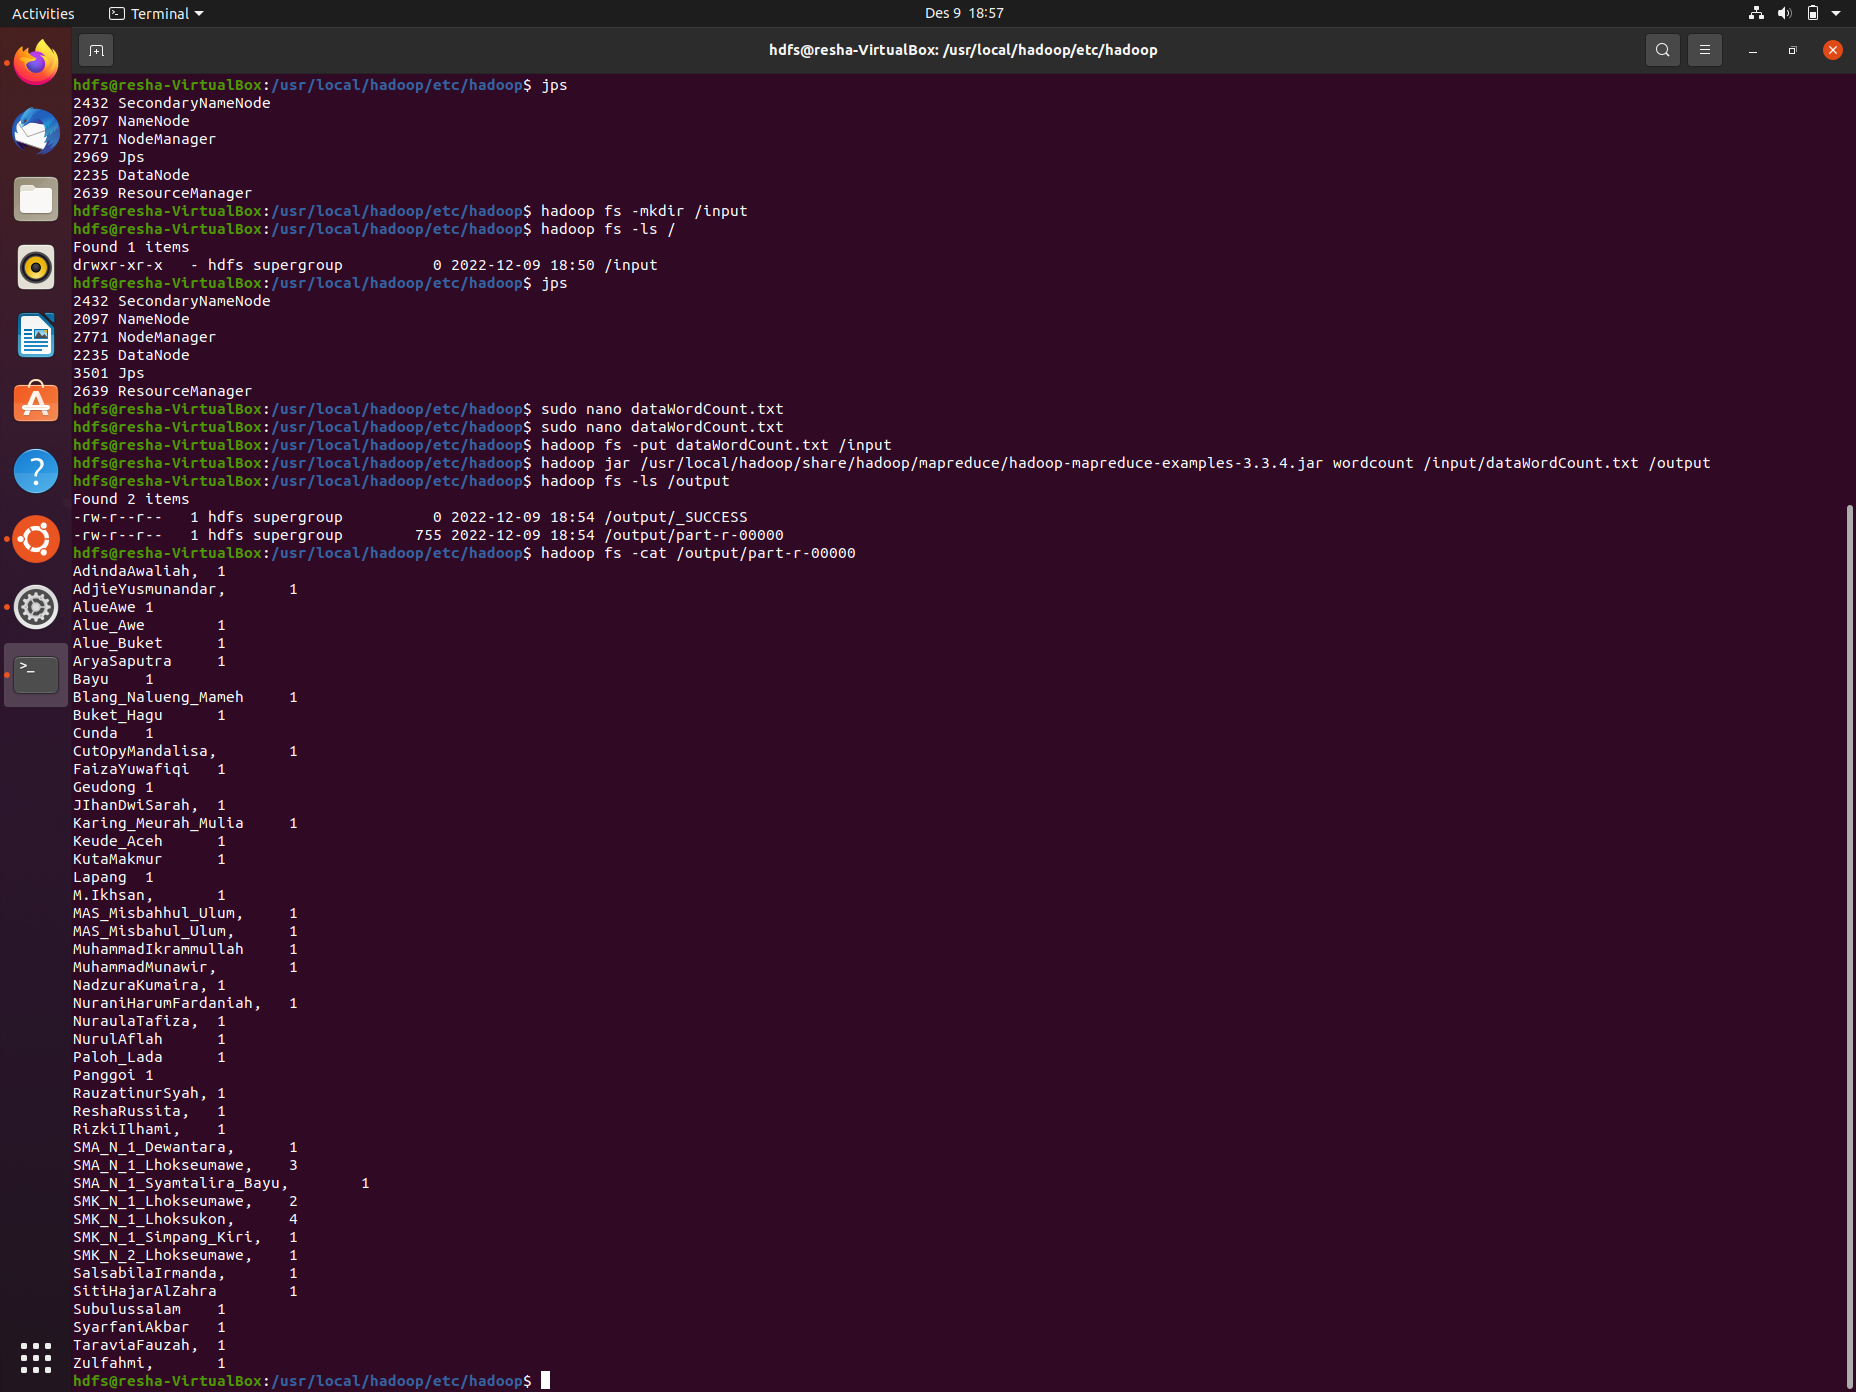
\includegraphics[width=.9\textwidth]{ReshaRussita/langkah6dan7-resha}
\caption{Hasil perhitungan WordCount bawaan Hadoop berdasarkan data output}
\label{gam:perkuliahan-08-12}
\end{figure}

\item Kesimpulan
\newline Pada Hadoop terdapat program untuk menghitung jumlah kata (WordCount) yang ada pada data. Untuk menghitung jumlah kata, saya sebagai praktikan melakukan input data terlebih dahulu, kemudian memprosesnya, sehingga menghasilkan data output. Data output tersebut yang digunakan untuk Hadoop menjalankan programnya yaitu WordCount.
Data yang saya input disini adalah data mahasiswa (nama, asal sekolah, dan alamat). Saat melihat hasil perhitungan pada data output, akan ditampilkan jumlah kata dari tiap-tiap nama, asal sekolah, dan alamat mahasiswa.

\end{enumerate}

\newday{\textbf{9 Desember 2022} - WordCount dengan Java}
\begin{enumerate}
\item Kendala dan Solusi
\newline Pada program WordCount bawaan Java, tidak ada kendala yang saya alami.

\begin{figure}[!ht]
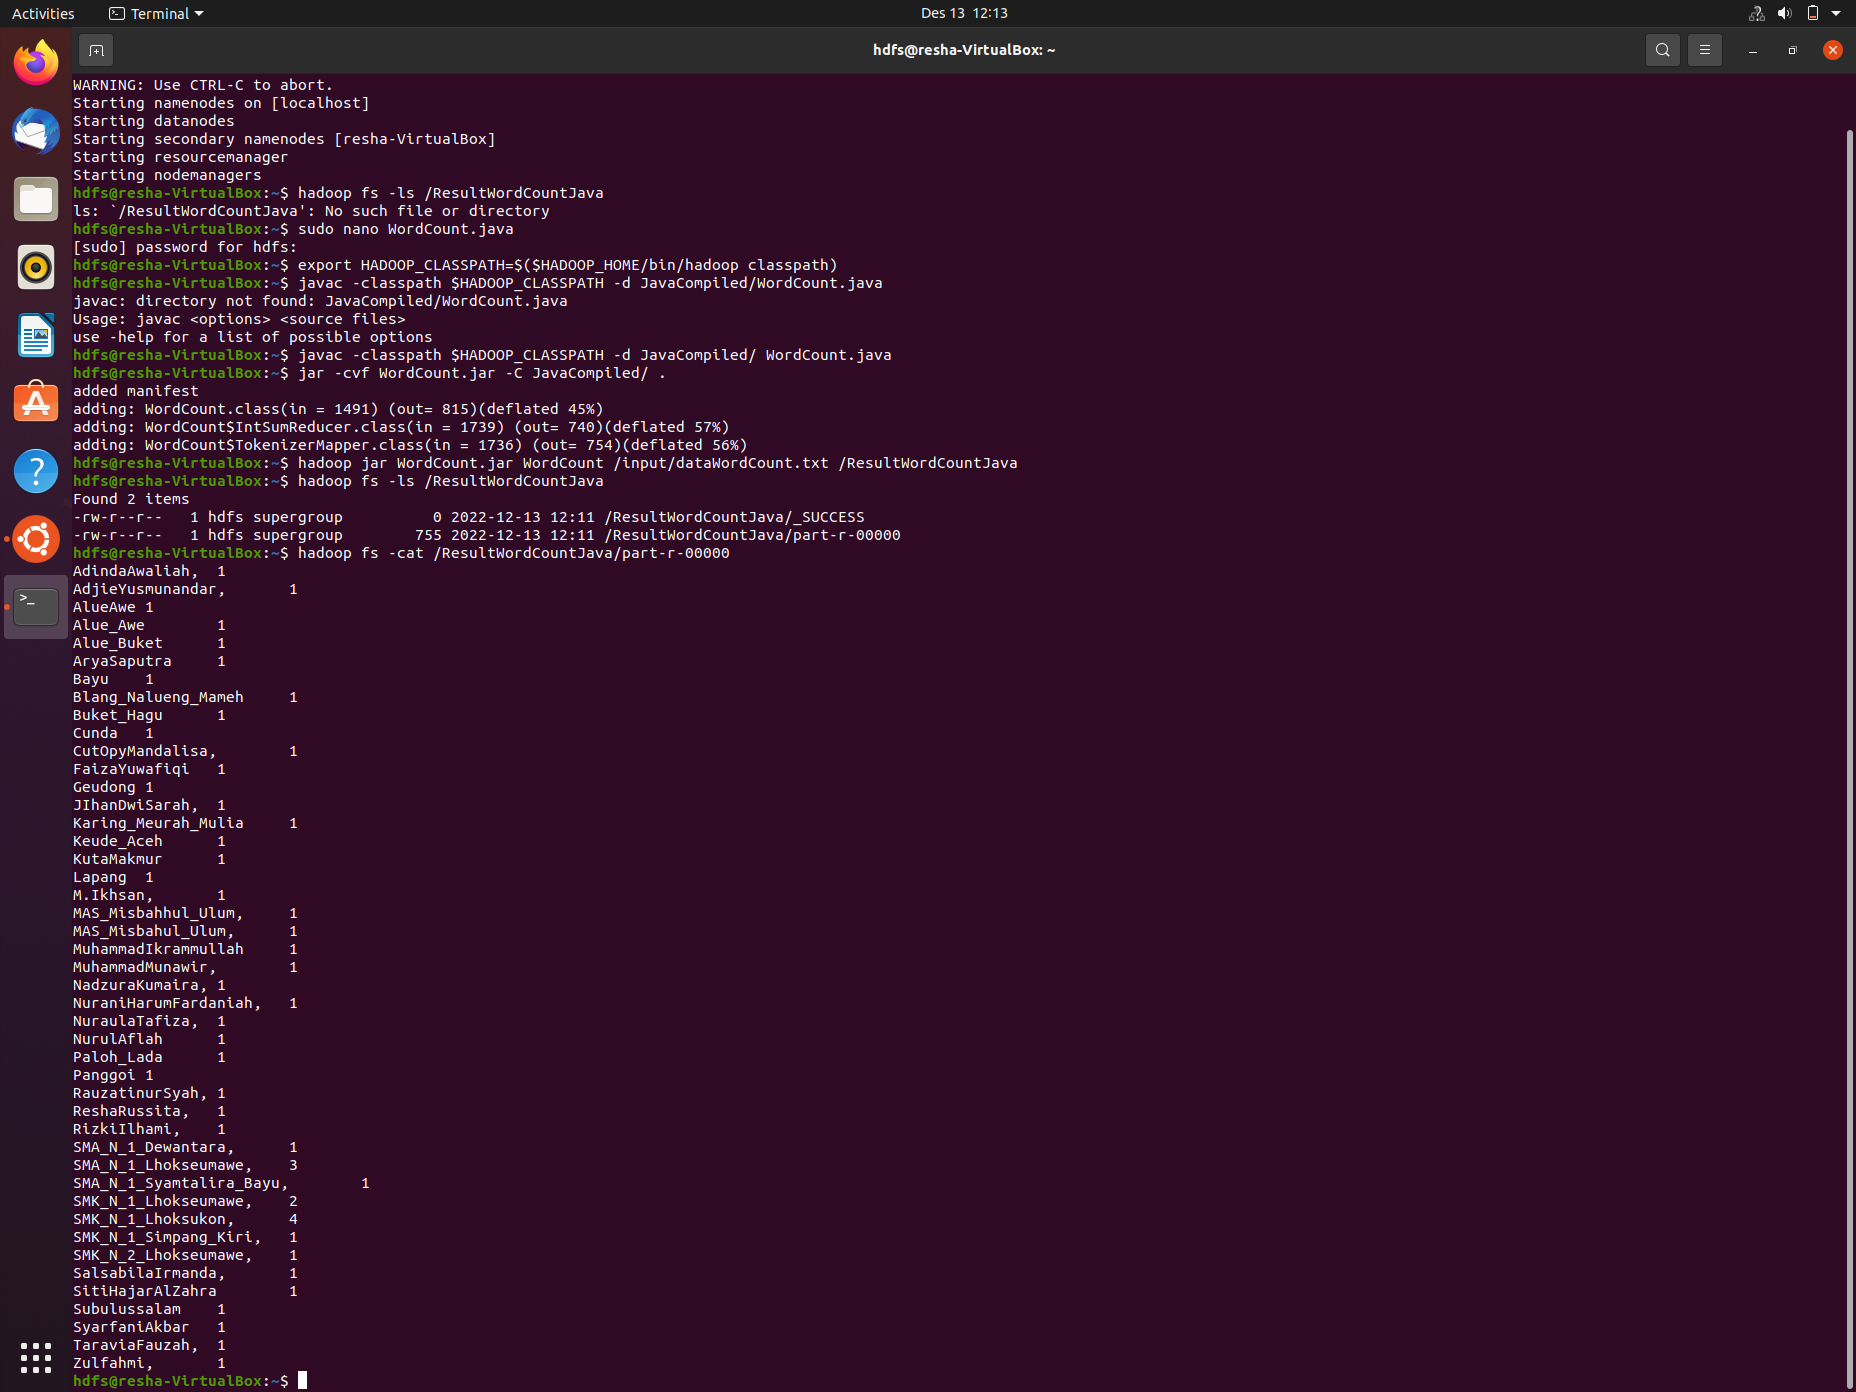
\includegraphics[width=.9\textwidth]{ReshaRussita/langkah9dan10-resha}
\caption{Hasil perhitungan WordCount dengan Java berdasarkan data output}
\label{gam:perkuliahan-08-12}
\end{figure}

\item Kesimpulan
\newline Praktikum ini yaitu menghitung jumlah kata (WordCount) yang ada pada data Java. Proses yang dijalankan mulai dari membuat program dan menyiapkan data untuk WordCount java, kemudian meng-compile program. Program yang dihasilkan sama seperti yang ditampilkan pada WordCount bawaan Hadoop.
\end{enumerate}

\newday{\textbf{15 Desember 2022}}
\begin{enumerate}
\item Kendala dan Solusi
% jelaskan kendala dan penyebab yang dialami saat mengikuti praktikum serta solusi atau langkah-langkah yang telah dilakukan

\item Kesimpulan
% berikan kesimpulan dari praktikum yang telah dikerjkan

\end{enumerate}
